\chapter{量子统计的表述}

\section{量子力学中的统计理论：密度矩阵}\label{ux91cfux5b50ux529bux5b66ux4e2dux7684ux7edfux8ba1ux7406ux8bbaux5bc6ux5ea6ux77e9ux9635}

我们考虑一组由 \(\mathcal{N}\) 个相同系统构成的集合，其中 \(\mathcal{N} \gg 1\)。这些系统具有共同的哈密顿算符，该算符可记作 \(\hat{H}\)。在时间 \(t\)，集合中各系统的物理状态将由波函数 \(\psi(\boldsymbol{r}_i,t)\) 描述，其中 \(\boldsymbol{r}_i\) 表示与所研究系统相关的坐标位置。设 \(\psi^k(\boldsymbol{r}_i,t)\) 表示在时间 \(t\) 时，集合中第 \(k\) 个系统恰好处于的物理状态的归一化波函数；自然地，\(k=1,2,\ldots,\mathcal{N}\)。函数 \(\psi^k(t)\) 的时间演化将由

薛定谔方程\(^{1}\)

\begin{equation}\tag{5.1.1}\label{eq:5.1.1}
\hat { H } \psi ^{k} ( t ) = i \hbar \dot { \psi } ^{k} ( t ) .
\end{equation}

引入一组完备的正交函数 \(\phi_{n}\)，波函数 \(\psi^{k}(t)\) 可以写成

\begin{equation}\tag{5.1.2}\label{eq:5.1.2}
\psi ^{k} ( t ) = \sum _ { n } a _ { n } ^{k} ( t ) \phi _ { n } ,
\end{equation}

其中

\begin{equation}\tag{5.1.3}\label{eq:5.1.3}
a _ { n } ^{k} ( t ) = \int \phi _ { n } ^{*} \psi ^{k} ( t ) d \tau ;
\end{equation}

在这里，\(\phi_{n}^{*}\) 表示 \(\phi_{n}\) 的复共轭，而 \(d\tau\) 则表示给定系统坐标空间的体积元素。显然，第 \(k\) 个系统的物理状态，同样可以用系数 \(a_{n}^{k}(t)\) 来描述。这些系数的时间演化将由

\begin{equation}\tag{5.1.4}\label{eq:5.1.4}
\begin{array}{rl} & { i \hbar \dot { a } _ { n } ^{k} ( t ) = i \hbar \int \phi _ { n } ^{*} \dot { \psi } ^{k} ( t ) d \tau = \int \phi _ { n } ^{*} \hat { H } \psi ^{k} ( t ) d \tau } \\& {  = \int \phi _ { n } ^{*} \hat { H } \Big \{ \sum _ { m } a _ { m } ^{k} ( t ) \phi _ { m } \Big \} d \tau } \\& {  = \sum _ { m } H _ { n m } a _ { m } ^{k} ( t ) , } \end{array}
\end{equation}

其中

\begin{equation}\tag{5.1.5}\label{eq:5.1.5}
H _ { n m } = \int \phi _ { n } ^{*} \hat { H } \phi _ { m } d \tau .
\end{equation}

系数 \(a_{n}^{k}(t)\) 的物理意义从\autoref{eq:5.1.2} 中便显而易见。它们是集合中各系统处于不同状态 \(\phi_{n}\) 的概率幅；从实际应用的角度来看，数值 \(|a_{n}^{k}(t)|^{2}\) 表示在时间 \(t\) 进行测量时，集合中第 \(k\) 个系统恰好处于特定状态 \(\phi_{n}\) 的概率。显然，我们必须有

\begin{equation}\tag{5.1.6}\label{eq:5.1.6}
\sum _ { n } | a _ { n } ^{k} ( t ) | ^{2} = 1  { \mathrm { ( f o r ~ a l l ~ } } k { \mathrm { ) } } .
\end{equation}

现在我们引入密度算符 \(\hat{\rho}(t)\)，其定义为矩阵元

\begin{equation}\tag{5.1.7}\label{eq:5.1.7}
\rho _ { m n } ( t ) = \frac { 1 } { \mathcal { N } } \sum _ { k = 1 } ^{\mathcal { N} } \left\{ a _ { m } ^{k} ( t ) a _ { n } ^{k *} ( t ) \right\} ;
\end{equation}

显然，矩阵元 \(\rho_{mn}(t)\) 是集合中 \(a_{m}(t)a_{n}^{*}(t)\) 量的平均值，而这一量在集合中的各个成员之间通常会有所差异。特别是，对角元 \(\rho_{nn}(t)\) 是集合中概率 \(|a_{n}(t)|^{2}\) 的平均值，后者

本身即为（量子力学）意义上的平均值。因此，我们在此遇到了一种双重平均过程------一次源于波函数的概率性因素，另一次源于集合的统计性因素。现在，量 \(\rho_{nn}(t)\) 表示，在时间 \(t\) 时，从集合中随机选取的一个系统，恰好处于状态 \(\phi_{n}\) 的概率。鉴于\autoref{eq:5.1.6} 和\autoref{eq:5.1.7}，

\begin{equation}\tag{5.1.8}\label{eq:5.1.8}
\sum _ { n } \rho _ { n n } = 1 .
\end{equation}

现在，我们来确定密度矩阵 \(\rho_{mn}(t)\) 的运动方程。借助于上述方程，我们得到：

\begin{equation}\tag{5.1.9}\label{eq:5.1.9}
\begin{array}{rl} & { i \hbar \dot { \rho } _ { m n } ( t ) = \frac { 1 } { \mathcal { N } } \sum _ { k = 1 } ^{\mathcal { N} } \Big [ i \hbar \Big \{ \dot { a } _ { m } ^{k} ( t ) a _ { n } ^{k *} ( t ) + a _ { m } ^{k} ( t ) \dot { a } _ { n } ^{k *} ( t ) \Big \} \Big ] } \\& {  = \frac { 1 } { \mathcal { N } } \sum _ { k = 1 } ^{\mathcal { N} } \Big [ \Big \{ \sum _ { l } H _ { m l } a _ { l } ^{k} ( t ) \Big \} a _ { n } ^{k *} ( t ) - a _ { m } ^{k} ( t ) \Big \{ \sum _ { l } H _ { n l } ^{*} a _ { l } ^{k *} ( t ) \Big \} \Big ] } \\& {  = \sum _ { l } \{ H _ { m l } \rho _ { l n } ( t ) - \rho _ { m l } ( t ) H _ { l n } \} } \\& {  = ( \hat { H } \hat { \rho } - \hat { \rho } \hat { H } ) _ { m n } ; } \end{array}
\end{equation}

在此，我们利用了这样一个事实：鉴于算符 \(\hat{H}\) 具有厄米性，即 \(H_{nl}^{*}=H_{ln}\)。运用对易关系的记法，方程（9）可写为

\begin{equation}\tag{5.1.10}\label{eq:5.1.10}
i \hbar \dot { \hat { \rho } } = [ \hat { H } , \hat { \rho } ] _ { - } .
\end{equation}

方程（10）是洛伊维尔经典方程（2.2.10）在量子力学中的类比。正如我们所预期的那样，从经典运动方程过渡到其量子力学对应形式时，泊松括号 \([\rho,H]\) 已被对易算符 \((\hat{\rho}\hat{H}-\hat{H}\hat{\rho})/i\hbar\) 所取代。

如果已知给定系统处于平衡态，则相应的系综必须是静止的，即 \(\dot{\rho}_{mn}=0\)。因此，方程（9）和（10）告诉我们：要使这一条件成立，首先，密度算符 \(\hat{\rho}\) 必须明确地依赖于哈密顿算符 \(\hat{H}\)（因为此时这两个算符必然对易）；其次，哈密顿算符不得显式地依赖于时间，也就是说，我们必须满足以下两个条件：一是 \(\hat{\rho}=\hat{\rho}(\hat{H})\)；二是 \(\dot{\hat{H}}=0\)。若基函数 \(\phi_{n}\) 是哈密顿算符本身的本征函数，则矩阵 \(H\) 和 \(\rho\) 将会是对角矩阵：

\begin{equation}\tag{5.1.11}\label{eq:5.1.11}
H _ { m n } = E _ { n } \delta _ { m n } ,  \varrho _ { m n } = \varrho _ { n } \delta _ { m n } .
\end{equation}

² 请注意，在这种（所谓的能量）表示法中，密度算符 \(\hat{\rho}\) 可以写成

\begin{equation}\tag{5.1.12}\label{eq:5.1.12}
\hat { \rho } = \sum _ { n } | \phi _ { n } \rangle \rho _ { n } \langle \phi _ { n } | ,
\end{equation}

则

\begin{equation}\tag{5.1.13}\label{eq:5.1.13}
\rho _ { k l } = \sum _ { n } \langle \phi _ { k } | \phi _ { n } \rangle \rho _ { n } \langle \phi _ { n } | \phi _ { l } \rangle = \sum _ { n } \delta _ { k n } \rho _ { n } \delta _ { n l } = \rho _ { k } \delta _ { k l } .
\end{equation}

对角元素 \(\rho_{n}\) 作为衡量标准，用于描述从系综中随机选取（且任意时刻）的系统，最终落入本征态 \(\phi_{n}\) 中的概率；因此，\(\rho_{n}\) 自然会依赖于哈密顿算符对应的本征值 \(E_{n}\)。然而，这种依赖性的具体性质，却取决于我们希望构建的系综的``类型''。

在除能量表示法之外的任何其他表示法中，密度矩阵可能为对角矩阵，也可能不是。不过，一般来说，密度矩阵总是对称的：

\begin{equation}\tag{5.1.14}\label{eq:5.1.14}
\rho _ { m n } = \rho _ { n m } .
\end{equation}

之所以存在这种对称性，其物理原因在于：在统计平衡状态下，物理系统从一种状态（在新表示法下）切换到另一种状态的倾向，必须与同样强烈的趋势相抗衡------即在相反方向上从同一状态之间进行切换。这一细致平衡的条件，对于维持系综内部的平衡分布至关重要。

最后，我们来考虑某一物理量 \(G\) 的期望值，该物理量在动力学上由算符 \(\hat{G}\) 表示。其值将为

\begin{equation}\tag{5.1.15}\label{eq:5.1.15}
\langle G \rangle = \frac { 1 } { \mathcal { N } } \sum _ { k = 1 } ^{\mathcal { N} } \int \psi ^{k *} \hat { G } \psi ^{k} d \tau .
\end{equation}

用系数 \(a_{n}^{k}\) 来表示，

\begin{equation}\tag{5.1.16}\label{eq:5.1.16}
\langle G \rangle = \frac { 1 } { \mathcal { N } } \sum _ { k = 1 } ^{\mathcal { N} } \left[ \sum _ { m , n } a _ { n } ^{k *} a _ { m } ^{k} G _ { n m } \right] ,
\end{equation}

其中

\begin{equation}\tag{5.1.17}\label{eq:5.1.17}
G _ { n m } = \int \phi _ { n } ^{*} \hat { G } \phi _ { m } d \tau .
\end{equation}

引入密度矩阵 \(\rho\)，式（15）变为

\begin{equation}\tag{5.1.18}\label{eq:5.1.18}
\langle G \rangle = \sum _ { m , n } \rho _ { m n } G _ { n m } = \sum _ { m } ( \hat { \rho } \hat { G } ) _ { m m } = \mathrm { T r } ( \hat { \rho } \hat { G } ) .
\end{equation}

取 \(\hat{G}=\hat{1}\)，其中 \(\hat{1}\) 为单位算子，我们得到

\begin{equation}\tag{5.1.19}\label{eq:5.1.19}
\operatorname { T r } ( { \hat { \rho } } ) = 1 ,
\end{equation}

这与式（8）完全相同。需要指出的是，如果原始波函数 \(\psi^{k}\) 没有进行归一化处理，则期望值 \(\langle G \rangle\) 将由以下公式给出

\begin{equation}\tag{5.1.20}\label{eq:5.1.20}
\langle G \rangle = \frac { \mathrm { T r } ( \hat { \rho } \hat { G } ) } { \mathrm { T r } ( \hat { \rho } ) }
\end{equation}

相反。鉴于式（17）和式（19）的数学结构，任何物理量 \(G\) 的期望值显然与基 \(\{\phi_n\}\) 的选择无关------而这正是其应有的性质。

\section{各种统计系综的统计特性}\label{ux5404ux79cdux7edfux8ba1ux7cfbux7efcux7684ux7edfux8ba1ux7279ux6027}

\section{微正则系综}\label{a-ux5faeux89c2ux7edfux8ba1ux7cfbux7efc}

微正则系综的构建基于这样一个前提：构成该系综的系统具有固定粒子数 \(N\)、固定体积 \(V\)，以及位于区间 \((E-\frac{1}{2}\Delta, E+\frac{1}{2}\Delta)\) 内的能量，其中 \(\Delta \ll E\)。系统可达到的微态总数用符号 \(\Gamma(N,V,E;\Delta)\) 表示，并且根据假设，这些微态中的任意一个都与其他微态出现的概率相同。这一假设以公理形式纳入理论中，通常称为“各可及状态的先验等概率公理”。

因此，密度矩阵 \(\rho_{mn}\)（在能量表示法下，必须是对角矩阵）将呈现如下形式

\begin{equation}\tag{5.2.1}\label{eq:5.2.1}
\rho _ { m n } = \rho _ { n } \delta _ { m n } ,
\end{equation}

其中

\begin{equation}\tag{5.2.2}\label{eq:5.2.2}
\rho _ { n } = \left\{ \begin{array}{ll} { 1 / \, \Gamma } & { \mathrm { f o r ~ e a c h ~ o f ~ t h e ~ a c c e s s i b l e ~ s t a t e s , } } \\{ 0 } & { \mathrm { f o r ~ a l l ~ o t h e r ~ s t a t e s ; } } \end{array} \right.
\end{equation}

归一化条件 \((5.1.18)\) 显然已得到满足。正如我们已经知道的那样，系统的热力学完全由其熵的表达式决定，而熵又由以下公式给出

\begin{equation}\tag{5.2.3}\label{eq:5.2.3}
S = k \ln \Gamma .
\end{equation}

由于总共有多少个不同的、可到达的微态 \(\Gamma\)，本应通过量子力学的方法来计算------从一开始就充分考虑了粒子的不可区分性------因此，如今不再会像吉布斯那样的悖论产生。此外，如果系统的量子态确实唯一无二（\(\Gamma=1\)），那么系统的熵也将完全消失。这为我们提供了坚实的理论基础，使我们得以推导出此前仅依赖经验的奈尔斯特定理（亦称热力学第三定律）。

通常将\(\Gamma=1\)情形下的情况称为纯态情形。在这种情况下，构建一个集合基本上是多余的，因为集合中的每一个系统都必须处于同一状态。因此，只存在一个非零的对角元素\(\rho_{nn}\)（实际上等于1），而其余所有元素均为零。该

因此，密度矩阵满足以下关系

\begin{equation}\tag{5.2.4}\label{eq:5.2.4}
\rho ^{2} = \rho .
\end{equation}

在另一种表示形式下，纯态情形将对应于

\begin{equation}\tag{5.2.5}\label{eq:5.2.5}
\rho _ { m n } = \frac { 1 } { \mathcal { N } } \sum _ { k = 1 } ^{\mathcal { N} } a _ { m } ^{k} a _ { n } ^{k *} = a _ { m } a _ { n } ^{*}
\end{equation}

因为现在所有\(k\)的取值在字面上是等价的。于是我们得到

\begin{equation}\tag{5.2.6}\label{eq:5.2.6}
\begin{array}{rl} & { \rho _ { m n } ^{2} = \sum _ { l } \rho _ { m l } \rho _ { l n } = \sum _ { l } a _ { m } a _ { l } ^{*} a _ { l } a _ { n } ^{*} } \\& {  = a _ { m } a _ { n } ^{*}  \left( \mathrm { b e c a u s e } \sum _ { l } a _ { l } ^{*} a _ { l } = 1 \right) } \\& {  = \rho _ { m n } . } \end{array}
\end{equation}

因此，\autoref{eq:5.2.4}在所有表示形式中均成立。

当\(\Gamma > 1\)时的情形通常被称为混合态情形。在能表示中，密度矩阵由\autoref{eq:5.2.1}和\autoref{eq:5.2.2}给出。如果我们现在转而采用任何其他表示形式，密度矩阵的一般形式应保持不变，即：(i) 对角元素仍应为零；(ii) 在允许的取值范围内，对角元素彼此应相等。然而，如果我们在一开始就以不同于能表示的其他表示形式来构建我们的集合，那么我们又如何能够从头开始就预见到密度矩阵的性质(i)呢？而性质(ii)却可以通过先验概率相等这一公理轻松推导出来呢？为了确保性质(i)以及性质(ii)在每一种表示形式中都成立，我们必须再引入另一条公理------即关于概率幅\(a_{n}^{k}\)的先验随机相位公理。而这又意味着，对于所有的\(k\)，波函数\(\psi^{k}\)都是基\(\{\phi_{n}\}\)的非相干叠加态。由于这一公理与先验概率相等公理的共同作用，在任何表示形式中，

\begin{equation}\tag{5.2.7}\label{eq:5.2.7}
\begin{array}{rlr} & { } & { \rho _ { m n } \equiv \frac { 1 } { \mathcal { N } } \sum _ { k = 1 } ^{\mathcal { N} } a _ { m } ^{k} a _ { n } ^{k *} = \frac { 1 } { \mathcal { N } } \sum _ { k = 1 } ^{\mathcal { N} } | a | ^{2} e ^{i \left( \theta _ { m} ^{k} - \theta _ { n } ^{k} \right) } } \\& { } & { = c \left\langle e ^{i \left( \theta _ { m} ^{k} - \theta _ { n } ^{k} \right) } \right\rangle } \\& { } & { = c \delta _ { m n } , } \end{array}
\end{equation}

这正是微正则系综所应有的特性。

因此，与常规认知所预期的相反，要实现微正则系综所对应的物理状况，我们通常需要两个

与其只引入一条公理，不如引入两条公理！第二条公理完全源自量子力学，其目的在于确保各组成系统之间互不干扰（从而完全消除相关性）；而这一特性反过来又使我们能够逐一清晰地构想集合中每个系统的整体状态，且与其它系统完全分离、彼此独立。

\section{正则系综}\label{b-ux5e38ux89c4ux7cfbux7efc}

在这一集合中，单个系统的宏观状态由参数 \(N\)、\(V\) 和 \(T\) 确定；能量 \(E\) 现在成为一种可变的量。从该集合中随机选取一个系统，其能量为 \(E_r\) 的概率，由玻尔兹曼因子 \(\exp(-\beta E_r)\) 确定，其中 \(\beta = 1/kT\)；参见第 3.1 节和第 3.2 节。因此，在能量表示法中，密度矩阵被定义为

\begin{equation}\tag{5.2.8}\label{eq:5.2.8}
\rho _ { m n } = \rho _ { n } \delta _ { m n } ,
\end{equation}

与

\begin{equation}\tag{5.2.9}\label{eq:5.2.9}
\rho _ { n } = C \exp { ( - \beta E _ { n } ) } ;  n = 0 , 1 , 2 , \ldots
\end{equation}

常数 \(C\) 是由归一化条件（5.1.18）所确定的，据此，

\begin{equation}\tag{5.2.10}\label{eq:5.2.10}
C = \frac { 1 } { \sum _ { n } \exp { ( - \beta E _ { n } ) } } = \frac { 1 } { Q _ { N } ( \beta ) } ,
\end{equation}

其中 \(Q_{N}(\beta)\) 是系统的配分函数。鉴于方程（5.1.12），请参阅脚注 2，该集合中的密度算子可以写成

\begin{equation}\tag{5.2.11}\label{eq:5.2.11}
\begin{array}{rl} & { \hat { \rho } = \sum _ { n } | \phi _ { n } \rangle \frac { 1 } { Q _ { N } ( \beta ) } e ^{- \beta E n} \langle \phi _ { n } | } \\& { = \frac { 1 } { Q _ { N } ( \beta ) } e ^{- \beta \hat { H} } \sum _ { n } | \phi _ { n } \rangle \langle \phi _ { n } | } \\& { = \frac { 1 } { Q _ { N } ( \beta ) } e ^{- \beta \hat { H} } = \frac { e ^{- \beta \hat { H} } } { \mathrm { T r } \left( e ^{- \beta \hat { H} } \right) } , } \end{array}
\end{equation}

对于算子 \(\sum_{n}|\phi_{n}\rangle\langle\phi_{n}|\) 来说，它等同于单位算子。需要指出的是，方程（11）中算子 \(\exp(-\beta\hat{H})\) 表示的是

\begin{equation}\tag{5.2.12}\label{eq:5.2.12}
\sum _ { j = 0 } ^{\infty} ( - 1 ) ^{j} \frac { ( \beta \hat { H } ) ^{j} } { j ! } .
\end{equation}

物理量 \(G\) 的期望值 \(\langle G\rangle_{N}\)，即由算子 \(\hat{G}\) 所表征的物理量，现在可表示为

\begin{equation}\tag{5.2.13}\label{eq:5.2.13}
\begin{array}{r} { \langle G \rangle _ { N } = \mathrm { T r } ( \hat { \rho } \hat { G } ) = \frac { 1 } { Q _ { N } ( \beta ) } \mathrm { T r } \big ( \hat { G } e ^{- \beta \hat { H} } \big ) } \\{ = \frac { \mathrm { T r } \big ( \hat { G } e ^{- \beta \hat { H} } \big ) } { \mathrm { T r } \big ( e ^{- \beta \hat { H} } \big ) } ; } \end{array}
\end{equation}

这里的后缀 \(N\) 强调了这一平均运算是在固定数量 \(N\) 的集合上进行的事实。

\section{巨正则系综}\label{c-ux5927ux5747ux503cux96c6ux5408}

在这一集合中，密度算子 \(\hat{\rho}\) 操作于一个具有不确定粒子数的希尔伯特空间。因此，密度算子不仅必须与哈密顿算子 \(\hat{H}\) commute，还必须与一个数算子 \(\hat{n}\) commute，而该数算子的本征值分别为 0、1、2\ldots\ldots。如今，可以通过对前一情形进行直接的推广，得到密度算子的精确形式，其结果是

\begin{equation}\tag{5.2.14}\label{eq:5.2.14}
\hat { \rho } = \frac { 1 } { Q ( \mu , V , T ) } e ^{- \beta ( \hat { H} - \mu \hat { n } ) } ,
\end{equation}

其中

\begin{equation}\tag{5.2.15}\label{eq:5.2.15}
\mathcal { Q } ( \mu , V , T ) = \sum _ { r , s } e ^{- \beta ( E _ { r} - \mu N _ { s } ) } = \mathrm { T r } \{ e ^{- \beta ( \hat { H} - \mu \hat { n } ) } \} .
\end{equation}

集合平均 \(\langle G\rangle\) 现在可表示为

\begin{equation}\tag{5.2.16}\label{eq:5.2.16}
\begin{array}{r} { \langle G \rangle = \frac { 1 } { Q ( \mu , V , T ) } \mathrm { T r } \big ( \hat { G } e ^{- \beta \hat { H} } e ^{\beta \mu \hat { n} } \big ) } \\{ = \frac { \displaystyle \sum _ { N = 0 } ^{\infty} z ^{N} \langle G \rangle _ { N } Q _ { N } ( \beta ) } { \displaystyle \sum _ { N = 0 } ^{\infty} z ^{N} Q _ { N } ( \beta ) } , } \end{array}
\end{equation}

其中 \(z(\equiv e^{\beta\mu})\) 是系统的 fugacity，而 \(\langle G\rangle_{N}\) 则是按方程（13）所给出的规范集合平均值。这些公式中出现的量 \(\mathcal{Q}(\mu,V,T)\) 显然就是系统的巨配分函数。

\section{示例}\label{ux793aux4f8b_chap5}

\section{磁场中的电子}\label{a-ux78c1ux573aux4e2dux7684ux7535ux5b50}

为了便于说明，我们考虑单个电子的情况------该电子具有自旋 \(\frac{1}{2}\hbar\hat{\sigma}\) 和磁矩 \(\mu_{B}\)，其中 \(\hat{\sigma}\) 是泡利自旋算子，而 \(\mu_{B}=e\hbar/2mc\)。

电子的自旋在施加的磁场\(B\)的参考方向上，可以有两种可能的取向：↑或↓。若将施加的磁场沿z轴方向定义，则自旋的构型哈密顿量可表示为：

\begin{equation}\tag{5.3.1}\label{eq:5.3.1}
\hat { H } = - \mu _ { B } ( \hat { \sigma } \cdot B ) = - \mu _ { B } B \hat { \sigma } _ { z } .
\end{equation}

在使\(\hat{\sigma}_{z}\)对角化的基底中，即

\begin{equation}\tag{5.3.2}\label{eq:5.3.2}
\hat { \sigma } _ { x } = \left( \begin{array}{ll} { 0 } & { 1 } \\{ 1 } & { 0 } \end{array} \right) ,  \hat { \sigma } _ { y } = \left( \begin{array}{ll} { 0 } & { - i } \\{ i } & { 0 } \end{array} \right) ,  \hat { \sigma } _ { z } = \left( \begin{array}{ll} { 1 } & { 0 } \\{ 0 } & { - 1 } \end{array} \right) ,
\end{equation}

在正则系综中，密度矩阵为

\begin{equation}\tag{5.3.3}\label{eq:5.3.3}
\begin{array}{rl} & { ( \hat { \rho } ) = \frac { \left( e ^{- \beta \hat { H} } \right) } { \mathrm { T r } \left( e ^{- \beta \hat { H} } \right) } } \\& { = \frac { 1 } { e ^{\beta \mu _ { B} B } + e ^{- \beta \mu _ { B} B } } \left( e ^{\beta \mu _ { B} B } \begin{array}{cc} { { 0 } } & { { 0 } } \\{ { 0 } } & { { e ^{- \beta \mu _ { B} B } } } \end{array} \right) . } \end{array}
\end{equation}

因此，我们得到\(\sigma_{z}\)的期望值为

\begin{equation}\tag{5.3.4}\label{eq:5.3.4}
\langle \sigma _ { z } \rangle = \mathrm { T r } ( \hat { \rho } \hat { \sigma } _ { z } ) = \frac { e ^{\beta \mu _ { B} B } - e ^{- \beta \mu _ { B} B } } { e ^{\beta \mu _ { B} B } + e ^{- \beta \mu _ { B} B } } = \mathrm { t a n h } ( \beta \mu _ { B } B ) ,
\end{equation}

与第3.9节和第3.10节的结论完全一致。

\section{箱内自由粒子}\label{b-ux7bb1ux5185ux81eaux7531ux7c92ux5b50}

现在我们来考虑质量为\(m\)的自由粒子，其处于边长为\(L\)的立方体箱中。该粒子的哈密顿量可表示为

\begin{equation}\tag{5.3.5}\label{eq:5.3.5}
\hat { H } = - \frac { \hbar ^{2} } { 2 m } \nabla ^{2} = - \frac { \hbar ^{2} } { 2 m } \left( \frac { \partial ^{2} } { \partial x ^{2} } + \frac { \partial ^{2} } { \partial y ^{2} } + \frac { \partial ^{2} } { \partial z ^{2} } \right) ,
\end{equation}

而满足周期性边界条件的哈密顿量的本征函数，

\begin{equation}\tag{5.3.6}\label{eq:5.3.6}
\begin{array}{r} { \phi ( x + L , y , z ) = \phi ( x , y + L , z ) = \phi ( x , y , z + L ) } \\{ = \phi ( x , y , z ) , } \end{array}
\end{equation}

由

\begin{equation}\tag{5.3.7}\label{eq:5.3.7}
\phi _ { E } ( r ) = \frac { 1 } { L ^{3 / 2} } \exp { ( i \boldsymbol { k } \cdot \boldsymbol { r } ) } ,
\end{equation}

对应的本征值\(E\)为

\begin{equation}\tag{5.3.8}\label{eq:5.3.8}
E = \frac { \hbar ^{2} k ^{2} } { 2 m } ,
\end{equation}

以及对应的波矢量\(k\)为

\begin{equation}\tag{5.3.9}\label{eq:5.3.9}
\pmb { k } \equiv ( k _ { x } , k _ { y } , k _ { z } ) = \frac { 2 \pi } { L } ( n _ { x } , n _ { y } , n _ { z } ) ;
\end{equation}

量子数\(n_{x}\)、\(n_{y}\)和\(n_{z}\)必须为整数（正整数、负整数或零）。用符号表示，我们可以写成

\begin{equation}\tag{5.3.10}\label{eq:5.3.10}
k = \frac { 2 \pi } { L } n ,
\end{equation}

其中\(n\)是一个具有整数分量\(0, \pm1, \pm2, \ldots\)的向量。

接下来，我们来计算该系统密度矩阵（\(\hat{\rho}\)）在正则系综中的表达式；我们采用坐标表示法计算。根据\autoref{eq:5.2.11}，我们有

\begin{equation}\tag{5.3.11}\label{eq:5.3.11}
\begin{array}{r} { \langle \pmb { r } | e ^{- \beta \hat { H} } | \pmb { r } ^{\prime} \rangle = \sum _ { E } \langle \pmb { r } | E \rangle e ^{- \beta E} \langle E | \pmb { r } ^{\prime} \rangle } \\{ = \sum _ { E } e ^{- \beta E} \phi _ { E } ( \pmb { r } ) \phi _ { E } ^{*} ( \pmb { r } ^{\prime} ) . } \end{array}
\end{equation}

将\autoref{eq:5.3.7}代入，并利用\autoref{eq:5.3.8}和\autoref{eq:5.3.10}，我们得到

\begin{equation}\tag{5.3.12}\label{eq:5.3.12}
\begin{array}{rl} & { \langle \pmb { r } | e ^{- \beta \hat { H} } | \pmb { r } ^{\prime} \rangle = \frac { 1 } { L ^{3} } \sum _ { k } \exp \left[ - \frac { \beta \hbar ^{2} } { 2 m } k ^{2} + i \pmb { k } \cdot ( \pmb { r } - \pmb { r } ^{\prime} ) \right] } \\& { \approx \frac { 1 } { ( 2 \pi ) ^{3} } \int \exp \left[ - \frac { \beta \hbar ^{2} } { 2 m } k ^{2} + i \pmb { k } \cdot ( \pmb { r } - \pmb { r } ^{\prime} ) \right] d ^{3} k } \\& { = \left( \frac { m } { 2 \pi \beta \hbar ^{2} } \right) ^{3 / 2} \exp \left[ - \frac { m } { 2 \beta \hbar ^{2} } | \pmb { r } - \pmb { r } ^{\prime} | ^{2} \right] ; } \end{array}
\end{equation}

参见附录B中的式(B.41)和式(B.42)。由此可知，

\begin{equation}\tag{5.3.13}\label{eq:5.3.13}
\begin{array}{rl} & { \mathrm { T r } ( e ^{- \beta \hat { H} } ) = \int \langle \mathbf { r } | e ^{- \beta \hat { H} } | \mathbf { r } \rangle d ^{3} r } \\& {  = V \left( \frac { m } { 2 \pi \beta \hbar ^{2} } \right) ^{3 / 2} . } \end{array}
\end{equation}

\autoref{eq:5.3.13}所表达的正是单个粒子在体积为\(V\)的箱中受限时的配分函数\(Q_{1}(\beta)\)；参见\autoref{eq:3.5.19}。将\autoref{eq:5.3.12}除以\autoref{eq:5.3.13}，我们得到在坐标表示法中密度矩阵的表达式

\begin{equation}\tag{5.3.14}\label{eq:5.3.14}
\langle \pmb { r } | \hat { \rho } | \pmb { r } ^{\prime} \rangle = \frac { 1 } { V } \exp \left[ - \frac { m } { 2 \beta \hbar ^{2} } | \pmb { r } - \pmb { r } ^{\prime} | ^{2} \right] .
\end{equation}

正如预期的那样，矩阵\(\rho_{r,r'}\)在状态\(r\)和状态\(r'\)之间是对称的。此外，对角元素\(\langle r|\rho|r\rangle\)代表了粒子处于

点 \(r\) 所处的邻域与 \(r\) 无关；这意味着，在单个自由粒子的情况下，盒内所有位置获得该粒子的概率是相等的。另一方面，非对角元 \(\langle r|\rho|r'\rangle\) 表示的是从位置坐标 \(r\) 到 \(r'\) 之间``自发跃迁''的概率，因此它也是衡量波包在距波包中心距离为 \(|r-r'|\) 处的相对``强度''的指标。波包的空间范围------即衡量粒子位置定位不确定性程度的参数------显然约为 \(\hbar/(mkT)^{1/2}\)；后者同时也是粒子平均热波长的度量。此处所发现的空间扩散纯属量子力学效应；毫不意外，它在高温下往往会趋于消失。事实上，随着 \(\beta\to0\)，\autoref{eq:5.3.14} 的行为会趋近于狄拉克函数，这表明我们又回到了经典理论中关于质点的描述。

最后，我们来确定哈密顿算符本身的期望值。根据\autoref{eq:5.3.5} 和\autoref{eq:5.3.14}，我们得到

\begin{equation}\tag{5.3.15}\label{eq:5.3.15}
\begin{array}{rl} & { \langle H \rangle = \mathrm { T r } ( \hat { H } \hat { \rho } ) = - \frac { \hbar ^{2} } { 2 m V } \int \left\{ \nabla ^{2} \exp \left[ - \frac { m } { 2 \beta \hbar ^{2} } | \boldsymbol { r } - \boldsymbol { r } ^{\prime} | ^{2} \right] \right\} _ { r = r ^{\prime} } d ^{3} r } \\& { = \frac { 1 } { 2 \beta V } \int \left\{ \left[ 3 - \frac { m } { \beta \hbar ^{2} } | \boldsymbol { r } - \boldsymbol { r } ^{\prime} | ^{2} \right] \exp \left[ - \frac { m } { 2 \beta \hbar ^{2} } | \boldsymbol { r } - \boldsymbol { r } ^{\prime} | ^{2} \right] \right\} _ { r = r ^{\prime} } d ^{3} r } \\& { = \frac { 3 } { 2 \beta } = \frac { 3 } { 2 } k T , } \end{array}
\end{equation}

这确实符合预期。否则，

\begin{equation}\tag{5.3.16}\label{eq:5.3.16}
\langle H \rangle = \frac { \mathrm { T r } ( \hat { H } e ^{- \beta \hat { H} } ) } { \mathrm { T r } ( e ^{- \beta \hat { H} } ) } = - \frac { \partial } { \partial \beta } \ln \mathrm { T r } ( e ^{- \beta \hat { H} } )
\end{equation}

将此结果与\autoref{eq:5.3.13} 结合，便可得出相同的结论。

\section{线性谐振子}\label{c-ux7ebfux6027ux8c10ux632fux5b50}

接下来，我们来考虑线性谐振子的情况，其哈密顿算符由如下形式给出：

\begin{equation}\tag{5.3.17}\label{eq:5.3.17}
\hat { H } = - \frac { \hbar ^{2} } { 2 m } \frac { \partial ^{2} } { \partial q ^{2} } + \frac { 1 } { 2 } m \omega ^{2} q ^{2} ,
\end{equation}

具有本征值

\begin{equation}\tag{5.3.18}\label{eq:5.3.18}
E _ { n } = \left( n + \frac { 1 } { 2 } \right) \hbar \omega ;  n = 0 , 1 , 2 , \ldots
\end{equation}

以及本征函数

\begin{equation}\tag{5.3.19}\label{eq:5.3.19}
\phi _ { n } ( q ) = \left( \frac { m \omega } { \pi \hbar } \right) ^{1 / 4} \frac { H _ { n } ( \xi ) } { ( 2 ^{n} n ! ) ^{1 / 2} } e ^{- ( 1 / 2 ) \xi ^ { 2} } ,
\end{equation}

其中

\begin{equation}\tag{5.3.20}\label{eq:5.3.20}
\xi = \left( \frac { m \omega } { \hbar } \right) ^{1 / 2} q
\end{equation}

且

\begin{equation}\tag{5.3.21}\label{eq:5.3.21}
H _ { n } ( \xi ) = ( - 1 ) ^{n} e ^{\xi ^ { 2} } \left( \frac { d } { d \xi } \right) ^{n} e ^{- \xi ^ { 2} } .
\end{equation}

在 \(q\) 域中，算符 \(\exp(-\beta\hat{H})\) 的矩阵元可表示为

\begin{equation}\tag{5.3.22}\label{eq:5.3.22}
\begin{array}{rl} & { \langle q | e ^{- \beta \hat { H} } | q ^{\prime} \rangle = \displaystyle \sum _ { n = 0 } ^{\infty} e ^{- \beta E _ { n} } \phi _ { n } ( q ) \phi _ { n } ( q ^{\prime} ) } \\& {  = \left( \frac { m \omega } { \pi \hbar } \right) ^{1 / 2} e ^{- ( 1 / 2 ) ( \xi ^ { 2} + \xi ^{\prime 2} ) } \displaystyle \sum _ { n = 0 } ^{\infty} \left\{ e ^{- ( n + 1 / 2 ) \beta \hbar \omega} \frac { H _ { n } ( \xi ) H _ { n } ( \xi ^{\prime} ) } { 2 ^{n} n ! } \right\} . } \end{array}
\end{equation}

对 \(n\) 的求和运算在计算上略显复杂；然而，最终结果为\(^{3}\)

\begin{equation}\tag{5.3.23}\label{eq:5.3.23}
\begin{array}{r} { \langle q | \mathrm { e } ^{- \beta \hat { H} } | q ^{\prime} \rangle = \bigg [ \frac { m \omega } { 2 \pi \hbar \sinh ( \beta \hbar \omega ) } \bigg ] ^{1 / 2} } \\{ \times \exp \left[ - \frac { m \omega } { 4 \hbar } \left\{ ( q + q ^{\prime} ) ^{2} \operatorname { t a n h } \left( \frac { \beta \hbar \omega } { 2 } \right) + ( q - q ^{\prime} ) ^{2} \coth \left( \frac { \beta \hbar \omega } { 2 } \right) \right\} \right] , } \end{array}
\end{equation}

由此可得

\begin{equation}\tag{5.3.24}\label{eq:5.3.24}
\begin{array}{rl} & { \mathrm { T r } ( e ^{- \beta \hat { H} } ) = \int _ { - \infty } ^{\infty} \langle q | e ^{- \beta \hat { H} } | q \rangle d q } \\& {  = \left[ \frac { m \omega } { 2 \pi \hbar \sinh ( \beta \hbar \omega ) } \right] ^{1 / 2} \int _ { - \infty } ^{\infty} \exp \left[ - \frac { m \omega q ^{2} } { \hbar } \operatorname { t a n h } \left( \frac { \beta \hbar \omega } { 2 } \right) \right] d q } \\& { = \frac { 1 } { 2 \sinh \left( \frac { 1 } { 2 } \beta \hbar \omega \right) } = \frac { e ^{- ( 1 / 2 ) \beta \hbar \omega} } { 1 - e ^{- \beta \hbar \omega} } . } \end{array}
\end{equation}

\autoref{eq:5.3.24} 确实是线性谐振子的配分函数；参见式（3.8.14）。与此同时，我们还发现，谐振子坐标位于接近数值 \(q\) 附近的概率密度为

\begin{equation}\tag{5.3.25}\label{eq:5.3.25}
\langle q | \hat { \rho } | q \rangle = \left[ \frac { m \omega \operatorname { t a n h } \left( \frac { 1 } { 2 } \beta \hbar \omega \right) } { \pi \hbar } \right] ^{1 / 2} \exp \left[ - \frac { m \omega q ^{2} } { \hbar } \operatorname { t a n h } \left( \frac { \beta \hbar \omega } { 2 } \right) \right] ;
\end{equation}

\(^{3}\) 该推导过程的数学细节可参见 Kubo（1965，第 175--177 页）。

我们注意到，这是一条在 \(q\) 方向上的高斯分布，其均值为零，方差为

\begin{equation}\tag{5.3.26}\label{eq:5.3.26}
q _ { \mathrm { r . m . s . } } = \left[ \frac { \hbar } { 2 m \omega \operatorname { t a n h } \left( \frac { 1 } { 2 } \beta \hbar \omega \right) } \right] ^{1 / 2} .
\end{equation}

概率分布（25）最早由布洛赫于1932年推导出来。在经典极限下（\(\beta\hbar\omega\ll1\)），该分布将完全趋于热力学分布------完全摆脱量子效应的影响：

\begin{equation}\tag{5.3.27}\label{eq:5.3.27}
\langle q | \hat { \rho } | q \rangle \approx \left( \frac { m \omega ^{2} } { 2 \pi k T } \right) ^{1 / 2} \exp \left[ - \frac { m \omega ^{2} q ^{2} } { 2 k T } \right] ,
\end{equation}

其分散度为\((kT/m\omega^2)^{1/2}\)。而在另一极端（\(\beta\hbar\omega\gg1\)），该分布将完全转变为量子力学分布------完全摆脱热力学效应的影响：

\begin{equation}\tag{5.3.28}\label{eq:5.3.28}
\langle q | \hat { \rho } | q \rangle \approx \left( \frac { m \omega } { \pi \hbar } \right) ^{1 / 2} \exp \left[ - \frac { m \omega q ^{2} } { \hbar } \right] ,
\end{equation}

其分散度为\((\hbar/2m\omega)^{1/2}\)。需要注意的是，极限分布（28）正是我们预期的、处于基态（\(n=0\)）的振子所对应的分布------即具有概率密度\(\phi_{0}^{2}(q)\)的分布；请参阅公式（19）至（21）。

鉴于振子的平均能量由以下公式给出：

\begin{equation}\tag{5.3.29}\label{eq:5.3.29}
\langle H \rangle = - \frac { \partial } { \partial \beta } \ln \mathrm { T r } \left( e ^{- \beta \hat { H} } \right) = \frac { 1 } { 2 } \hbar \omega \coth \left( \frac { 1 } { 2 } \beta \hbar \omega \right) ,
\end{equation}

我们注意到，分布（25）的温度依赖性仅由期望值\(\langle H\rangle\)决定。实际上，我们可以写出：

\begin{equation}\tag{5.3.30}\label{eq:5.3.30}
\langle q | \hat { \rho } | q \rangle = \left( \frac { m \omega ^{2} } { 2 \pi \langle H \rangle } \right) ^{1 / 2} \exp \left[ - \frac { m \omega ^{2} q ^{2} } { 2 \langle H \rangle } \right] ,
\end{equation}

其中

\begin{equation}\tag{5.3.31}\label{eq:5.3.31}
q _ { \mathrm { r . m . s . } } = \left( \frac { \langle H \rangle } { m \omega ^{2} } \right) ^{1 / 2} .
\end{equation}

现在我们很容易看出，振子的势能平均值（\(\frac{1}{2}m\omega^2q^2\)）等于\(\frac{1}{2}\langle H\rangle\)；相应地，其动能平均值（\(\frac{p^2}{2m}\)）也将保持一致。

5.4 由不可区分粒子组成的系统

接下来，我们将对由\(N\)个相同粒子组成的系统的量子力学描述进行阐述。为了便于理解，我们先考虑一个非相互作用粒子的气体；本研究的成果对于其他系统同样具有重要的参考意义。

如今，由\(N\)个非相互作用粒子组成的系统的哈密顿量，不过就是各单粒子哈密顿量之和：

\begin{equation}\tag{5.4.1}\label{eq:5.4.1}
\hat { H } ( q , p ) = \sum _ { i = 1 } ^{N} \hat { H } _ { i } ( q _ { i } , p _ { i } ) ;
\end{equation}

在这里，\((q_{i},p_{i})\)分别是第\(i\)个粒子的坐标与动量，而\(\hat{H}_{i}\)则是其哈密顿量。⁴ 由于这些粒子是相同的，因此哈密顿量\(\hat{H}_{i}\)（\(i=1,2,\ldots,N\)）在形式上完全相同；它们唯一的区别在于各自参数的取值。系统的非时间依赖薛定谔方程为：

\begin{equation}\tag{5.4.2}\label{eq:5.4.2}
\hat { H } \psi _ { E } ( \pmb { q } ) = E \psi _ { E } ( \pmb { q } ) ,
\end{equation}

其中\(E\)是哈密顿量的特征值，\(\psi_{E}(\boldsymbol{q})\)则是对应的特征函数。根据（1），我们可以写出薛定谔方程的一个直接解，即：

\begin{equation}\tag{5.4.3}\label{eq:5.4.3}
\psi _ { E } ( \pmb { q } ) = \prod _ { i = 1 } ^{N} u _ { \varepsilon _ { i } } ( q _ { i } ) ,
\end{equation}

其中

\begin{equation}\tag{5.4.4}\label{eq:5.4.4}
E = \sum _ { i = 1 } ^{N} \varepsilon _ { i } ;
\end{equation}

式（3）中的因子\(u_{\varepsilon_i}(q_i)\)是单粒子哈密顿量\(\hat{H}_i(q_i,p_i)\)的特征函数，其特征值为\(\varepsilon_i\)：

\begin{equation}\tag{5.4.5}\label{eq:5.4.5}
\hat { H } _ { i } u _ { \varepsilon _ { i } } ( q _ { i } ) = \varepsilon _ { i } u _ { \varepsilon _ { i } } ( q _ { i } ) .
\end{equation}

因此，给定系统的稳态可以借助构成该系统的单粒子状态来加以描述。一般来说，我们可以通过指定一组数值 \(\{n_i\}\) 来表示系统的某一特定状态；这表明，在由能量值 \(\varepsilon_i\) 表征的本征态中，存在 \(n_i\) 个粒子。显然，分布集

\(\{n_{i}\}\) 必须符合以下条件

\begin{equation}\tag{5.4.6}\label{eq:5.4.6}
\sum _ { i } n _ { i } = N
\end{equation}

并且

相应地，该状态的波函数可写为

\begin{equation}\tag{5.4.7}\label{eq:5.4.7}
\psi _ { E } ( \pmb { q } ) = \prod _ { m = 1 } ^{n _ { 1} } u _ { 1 } ( m )  \prod _ { m = n _ { 1 } + 1 } ^{n _ { 1} + n _ { 2 } } u _ { 2 } ( m ) \ldots ,
\end{equation}

其中，符号 \(u_{i}(m)\) 代表单粒子波函数 \(u_{\varepsilon_{i}}(q_{m})\)。

现在，假设我们在式（8）右侧所出现的坐标之间进行置换；结果，坐标 \((1,2,...,N)\) 将被替换为 \((P1,P2,...,PN)\)，例如。由此产生的波函数，我们可以称之为 \(P\psi_E(\boldsymbol{q})\)，将变为

\begin{equation}\tag{5.4.8}\label{eq:5.4.8}
P \psi _ { E } ( \pmb { q } ) = \prod _ { m = 1 } ^{n _ { 1} } u _ { 1 } ( P m ) \prod _ { m = n _ { 1 } + 1 } ^{n _ { 1} + n _ { 2 } } u _ { 2 } ( P m ) . . . .
\end{equation}

在经典物理学中，即使给定系统的粒子彼此相同，但它们仍被视为相互区分的；因此，任何能够将两个不同单粒子状态中的粒子进行互换的置换，都被认为导致了系统中一个新的、在物理上 distinct 的微观状态。例如，经典物理学认为，一个微观状态，其中所谓的第 5 个粒子处于状态 \(u_i\)，而所谓的第 7 个粒子处于状态 \(u_j\)（且 \(j \neq i\)），与一个微观状态------其中第 7 个粒子处于状态 \(u_i\)，而第 5 个粒子处于状态 \(u_j\)------是截然不同的。这导致了

\begin{equation}\tag{5.4.9}\label{eq:5.4.9}
\frac { N ! } { n _ { 1 } ! n _ { 2 } ! \ldots }
\end{equation}

（理论上）不同的系统微观状态，对应于给定的分布模式 \(\{n_i\}\)。此时，数字（10）将被赋予作为``统计权重因子''，用于分配集合 \(\{n_i\}\)。当然，吉布斯所采用的``修正''------这一修正已在第 1.5 节和第 1.6 节中予以讨论------会将这一权重因子降低至

\begin{equation}\tag{5.4.10}\label{eq:5.4.10}
W _ { c } \{ n _ { i } \} = \frac { 1 } { n _ { 1 } ! n _ { 2 } ! \ldots } .
\end{equation}

而要理解该``修正''的物理依据，唯一可行的方式，便是从粒子固有的不可区分性出发。

然而，根据量子物理学的观点，即便在纳入吉布斯的修正之后，情况仍然不尽如人意；因为严格来说，一次粒子的互换

在相同粒子之间，即便它们处于不同的单粒子态，也不应导致系统的全新微态！因此，若要恰当地考虑粒子的不可区分性，我们绝不能将``第5个''粒子处于状态 \(u_i\)、而``第7个''粒子处于状态 \(u_j\) 的微态，与``第7个''粒子处于状态 \(u_i\)、而``第5个''粒子处于状态 \(u_j\) 的微态视为截然不同------尽管 \(i \neq j\)。因为将粒子标记为第1号、第2号等，充其量只是一种方便之举，并非现实本身所决定的。换句话说，在描述给定系统某一特定状态时，真正重要的，只是那组数字 \(n_i\)，它告诉我们各个单粒子态 \(u_i\) 中分别有多少个粒子；至于``哪个粒子处于哪个单粒子态？''这一问题，根本无关紧要。

因此，只要 \(n_i\) 的数值保持不变，由 \(N\) 个粒子进行任意排列所得的所有微态，都应被视为同一微态。出于同样的原因，只要该分布集 \(\{n_i\}\) 并未因其他物理原因被禁止，与之对应的权重因子，无论 \(n_i\) 的具体数值为何，都应同等地等于一：

\begin{equation}\tag{5.4.11}\label{eq:5.4.11}
W _ { q } \{ n _ { i } \} \equiv 1 .
\end{equation}

事实上，若因某种物理原因，该分布集 \(\{n_i\}\) 被禁止，则该分布集的权重因子 \(W_q\) 应同等地等于零；例如，请参见式（19）。

与此同时，我们可称之为``玻尔兹曼型''的波函数，用符号 \(\psi_{\mathrm{Boltz}}(\boldsymbol{q})\) 表示，由于在描述由不可区分粒子组成的系统状态时，\(u_{i}\) 和 \(u_{j}\) 之间对参数的互换会导致波函数在数学上和物理上均与我们最初所使用的波函数有所不同，因此这种波函数并不适用。既然仅仅交换粒子坐标并不会导致系统的全新微态，那么波函数 \(\psi_{E}(\boldsymbol{q})\) 就必须以这样一种方式构建：在实际应用中，它对参数之间的任何互换都几乎不敏感。实现这一目标最简单的方法，是将所有 \(N!\) 个由式（8）经其参数间所有可能排列得到的函数，以线性组合的形式加以构造；当然，这种组合必须满足这样一个条件：当对其中的坐标进行排列时，波函数 \(\psi\) 与 \(P\psi\) 必须满足以下性质：

\begin{enumerate}
\def\labelenumi{\arabic{enumi}.}
\setcounter{enumi}{4}
\tightlist
\item
  值得一提的是，早在1905年，埃伦费斯特就指出，要得出普朗克关于黑体辐射的公式，就必须对各种分布集 \(\{n_{i}\}\) 都赋予相等的先验概率。
\end{enumerate}

\begin{equation}\tag{5.4.12}\label{eq:5.4.12}
| P \psi | ^{2} = | \psi | ^{2} .
\end{equation}

这带来了以下几种可能性：

\begin{equation}\tag{5.4.13}\label{eq:5.4.13}
P \psi = \psi  { \mathrm { f o r ~ a l l ~ } } P ,
\end{equation}

这意味着波函数在其所有参数中都是对称的，或者

\begin{equation}\tag{5.4.14}\label{eq:5.4.14}
P \psi = \left\{ \begin{array}{ll} { + \psi } & { \mathrm { i f ~ } P \mathrm { ~ i s ~ a n ~ e v e n ~ p e r m u t a t i o n , } } \\{ - \psi } & { \mathrm { i f ~ } P \mathrm { ~ i s ~ a n ~ o d d ~ p e r m u t a t i o n , } } \end{array} \right.
\end{equation}

这意味着波函数在其参数中是反对称的。我们分别将这些波函数称为\(\psi_{\mathrm{S}}\)和\(\psi_{\mathrm{A}}\)；它们的数学结构如下：

\begin{equation}\tag{5.4.15}\label{eq:5.4.15}
\psi _ { S } ( \pmb { q } ) = \mathrm { c o n s t . } \sum _ { P } P \psi _ { \mathrm { B o l t z } } ( \pmb { q } )
\end{equation}

并且

\begin{equation}\tag{5.4.16}\label{eq:5.4.16}
\psi _ { A } ( \pmb { q } ) = \mathrm { c o n s t . } \sum _ { P } \delta _ { P } P \psi _ { \mathrm { B o l t z } } ( \pmb { q } ) ,
\end{equation}

在\(\psi_{A}\)的表达式中，\(\delta_{P}\)根据排列\(P\)是偶数还是奇数，取+1或−1的值。

我们注意到，\(\psi_{A}(\boldsymbol{q})\)这一函数可以写成斯莱特行列式的形式：

\begin{equation}\tag{5.4.17}\label{eq:5.4.17}
\psi_A(\boldsymbol{q})=\mathrm{const.}\begin{vmatrix}u_i(1)&u_i(2)&\cdots&u_i(N)\\u_j(1)&u_j(2)&\cdots&u_j(N)\\.&.&\cdots&.\\.&.&\cdots&.\\.&.&\cdots&.\\u_l(1)&u_l(2)&\cdots&u_l(N)\end{vmatrix},
\end{equation}

其中，主对角线正是玻尔兹曼式的波函数，而展开式中的其他项则对应着各种不同的排列方式；在进行组合（17）时，正负号会自动出现，因为我们对行列式进行展开。当交换一对参数（也就是交换行列式中对应的两列）时，波函数\(\psi_{A}\)只是改变了其符号，而这正是其应有的性质。然而，如果两个或更多粒子恰好处于同一单粒子态，那么行列式中相应的行就会变得完全相同，波函数便会消失。这种状态在物理上根本无法实现。因此，我们得出结论：若一个由不可区分粒子构成的系统，其波函数具有反对称性，

\(^{6}\)偶数（奇数）排列是指，通过在参数之间进行偶数（奇数）次``配对交换''，即可从原始顺序得到的排列。例如，在六个排列中，

\begin{equation}\tag{5.4.18}\label{eq:5.4.18}
( 1 , 2 , 3 ) ,  ( 2 , 3 , 1 ) ,  ( 3 , 1 , 2 ) ,  ( 1 , 3 , 2 ) ,  ( 3 , 2 , 1 ) ,  \mathrm { a n d }  ( 2 , 1 , 3 ) ,
\end{equation}

在参数1、2和3的六种排列中，前三个是偶数排列，后三个则是奇数排列。显然，只要在任意两个参数之间进行一次交换，就属于奇数排列。

\(^{7}\)这与这样一个事实直接相关：如果我们对处于同一单粒子态的两个粒子进行交换，那么\(P\psi_{A}\)显然会与\(\psi_{A}\)完全一致。与此同时，如果\(P\psi_{A} = -\psi_{A}\)，那么\(\psi_{A}\)必然为零。

那么，该系统的所有粒子都必须处于不同的单粒子态------这一结果等同于电子的泡利不相容原理。

相反地，由遵循排除原理的粒子构成的统计系统，其波函数必须满足在各变量之间呈反对称性的条件。支配此类粒子行为的统计被称为费米-狄拉克统计，或简称费米统计；统计及其所构成的粒子本身则被称为费米子。对于这样的系统，其统计权重因子 \(W_{\text{F.D.}}\{n_{i}\}\) 在分布参数 \(n_{i}\) 为 0 或 1 时始终为 1；否则，该因子为 0：

\begin{equation}\tag{5.4.19}\label{eq:5.4.19}
W _ { \mathrm { F . D . } } \{ n _ { i } \} = \left\{ \begin{array}{ll} { 1 } & { \mathrm { i f }  \sum _ { i } n _ { i } ^{2} = N , } \\{ 0 } & { \mathrm { i f }  \sum _ { i } n _ { i } ^{2} > N . } \end{array} \right.
\end{equation}

对于那些具有对称波函数的系统，并不会出现此类问题：尤其是，我们对数值 \(n_i\) 的取值没有任何限制。支配此类系统行为的统计被称为玻色-爱因斯坦统计，或简称玻色统计；而构成这些系统的粒子本身则被称为玻色子。对于这样的系统，其权重因子 \(W_{\text{B.E.}}\{n_i\}\) 无论 \(n_i\) 的取值为何，都恒等于 1：

\begin{equation}\tag{5.4.20}\label{eq:5.4.20}
W _ { \mathrm { B . E . } } \{ n _ { i } \} = 1 ;  n _ { i } = 0 , 1 , 2 , \ldots .
\end{equation}

在此需要指出的是，某一特定种类粒子所遵循的统计规律与这些粒子的固有自旋之间存在着密切的联系。例如，自旋为整数的粒子（当然以 \(\hbar\) 为单位）遵循玻色-爱因斯坦统计，而自旋为半整数的粒子则遵循费米-狄拉克统计。第一类粒子的例子包括光子、声子、\(\pi\) 粒子、引力子、He\(^{4}\) 原子等；而第二类粒子则包括电子、核子（质子和中子）、\(\mu\) 粒子、中微子、He\(^{3}\) 原子等。

最后，必须强调的是，尽管我们在此基于对非相互作用系统的研究得出了相关结论，但这些基本结果同样适用于相互作用系统。一般来说，所需的波函数 \(\psi(\boldsymbol{q})\) 并不能用单粒子波函数 \(u_{i}(q_{m})\) 来表示；然而，它要么属于满足\autoref{eq:5.4.14} 的 \(\psi_{S}(\boldsymbol{q})\) 类型，要么属于满足\autoref{eq:5.4.15} 的 \(\psi_{A}(\boldsymbol{q})\) 类型。

需要注意的是，当满足 \(\sum_{i}n_{i}^{2}=N\) 这一条件时，所有 \(n_{i}\) 都只能是 0 或 1。另一方面，如果其中任何 \(n_{i}\) 大于 1，则 \(\sum_{i}n_{i}^{2}\) 的值将大于 \(N\)。

\section{自由粒子系统的密度矩阵与配分函数}\label{ux81eaux7531ux7c92ux5b50ux7cfbux7edfux7684ux5bc6ux5ea6ux77e9ux9635ux4e0eux914dux5206ux51fdux6570}

假设给定的系统由 \(N\) 个不可区分且彼此不相互作用的粒子组成，这些粒子被限制在体积为 \(V\) 的立方体盒中，并且该系统属于以温度参数 \(\beta\) 为特征的规范系综。在坐标表示下，该系统的密度矩阵将为\(^{10}\)

\begin{equation}\tag{5.4.21}\label{eq:5.4.21}
\langle \pmb { r } _ { 1 } , \ldots , \pmb { r } _ { N } | \hat { \rho } | \pmb { r } _ { 1 } ^{\prime} , \ldots , \pmb { r } _ { N } ^{\prime} \rangle = \frac { 1 } { Q _ { N } ( \beta ) } \langle \pmb { r } _ { 1 } , \ldots , \pmb { r } _ { N } | e ^{- \beta \hat { H} } | \pmb { r } _ { 1 } ^{\prime} , \ldots , \pmb { r } _ { N } ^{\prime} \rangle ,
\end{equation}

其中，\(Q_{N}(\beta)\) 是系统的配分函数：

\begin{equation}\tag{5.4.22}\label{eq:5.4.22}
Q _ { N } ( \beta ) = \mathrm { T r } ( e ^{- \beta \hat { H} } ) = \int \langle \pmb { r } _ { 1 } , \dots , \pmb { r } _ { N } | e ^{- \beta \hat { H} } | \pmb { r } _ { 1 } , \dots , \pmb { r } _ { N } \rangle d ^{3 N} r .
\end{equation}

为简洁起见，我们将向量 \(r_i\) 用字母 \(i\) 表示，而带撇号的向量 \(r'_i\) 则用 \(i'\) 表示。此外，设 \(\psi_E(1,\ldots,N)\) 为哈密顿算符的本征函数，后缀 \(E\) 代表相应的本征值。于是我们有

\begin{equation}\tag{5.4.23}\label{eq:5.4.23}
\langle 1 , \ldots , N | e ^{- \beta \hat { H} } | 1 ^{\prime} , \ldots , N ^{\prime} \rangle = \sum _ { E } e ^{- \beta E} \left[ \psi _ { E } ( 1 , \ldots , N ) \psi _ { E } ^{*} ( 1 ^{\prime} , \ldots , N ^{\prime} ) \right] ,
\end{equation}

求和范围涵盖所有可能的 \(E\) 值；请与\autoref{eq:5.3.11} 进行对比。

由于构成给定系统的粒子彼此不相互作用，我们可以将本征函数 \(\psi_{E}(1,\ldots,N)\) 和本征值 \(E\) 分别用单粒子波函数 \(u_{i}(m)\) 以及单粒子能量 \(\varepsilon_{i}\) 来表示。此外，我们发现，最好以波矢量 \(\boldsymbol{k}_{i}\) 来进行计算，而非使用能量 \(\varepsilon_{i}\)；因此我们写作

\begin{equation}\tag{5.4.24}\label{eq:5.4.24}
E = \frac { \hbar ^{2} K ^{2} } { 2 m } = \frac { \hbar ^{2} } { 2 m } ( k _ { 1 } ^{2} + k _ { 2 } ^{2} + \cdots + k _ { N } ^{2} ) ,
\end{equation}

其中，右侧的 \(k_{i}\) 是各独立粒子的波矢量。在施加周期性边界条件的情况下，归一化的单粒子波函数为

\begin{equation}\tag{5.4.25}\label{eq:5.4.25}
u _ { k } ( \pmb { r } ) = V ^{- 1 / 2} \exp \{ i ( \pmb { k } \cdot \pmb { r } ) \} ,
\end{equation}

其中，

\begin{equation}\tag{5.4.26}\label{eq:5.4.26}
k = 2 \pi V ^{- 1 / 3} n ;
\end{equation}

在此，\(\boldsymbol{n}\) 表示一个三维向量，其各分量取值为 \(0, \pm1, \pm2, \ldots\)。那么，整个系统的波函数 \(\psi\) 将是，参见\autoref{eq:5.4.16}

并且 \((5.4.17)\)，

\begin{equation}\tag{5.4.27}\label{eq:5.4.27}
\psi _ { K } ( 1 , \ldots , N ) = ( N ! ) ^{- 1 / 2} \sum _ { P } \delta _ { P } P \{ u _ { k _ { 1 } } ( 1 ) \ldots u _ { k _ { N } } ( N ) \} ,
\end{equation}

其中，各 \(k_{i}\) 的模长满足如下条件：

\begin{equation}\tag{5.4.28}\label{eq:5.4.28}
( k _ { 1 } ^{2} + \cdots + k _ { N } ^{2} ) = K ^{2} .
\end{equation}

在 \(\psi_{K}\) 的表达式中，若粒子为玻色子，则 \(\delta_{P}\) 的值恒等于 +1；而对于费米子，则根据排列 \(P\) 是偶数还是奇数，\(\delta_{P}\) 的值则为 +1 或 -1。因此，从广义上讲，我们可以写成

\begin{equation}\tag{5.4.29}\label{eq:5.4.29}
\delta _ { P } = ( \pm 1 ) ^{[ P ]} ,
\end{equation}

其中，{[}P{]} 表示排列的顺序；请注意，该表达式中的上标符号适用于玻色子，而下标符号则适用于费米子。此处引入 \((N!)^{-1/2}\) 因子，旨在确保总波函数的归一化。

现在，无论排列 \(P\) 是作用于坐标 \(1,\ldots,N\)，还是作用于波矢量 \(k_1,\ldots,k_N\)，对波函数 (7) 都没有影响，毕竟我们最终是要对全部 \(N!\) 种排列进行求和。将经过排列的坐标记作 \(P1,\ldots,PN\)，将经过排列的波矢量记作 \(Pk_1,\ldots,Pk_N\)，则式（5.5.7） 可以写成

\begin{equation}\tag{5.4.30}\label{eq:5.4.30}
\begin{array}{rlr} & { } & { \psi _ { K } ( \mathbf { 1 } , \ldots , N ) = ( N ! ) ^{- 1 / 2} \sum _ { P } \delta _ { P } \left\{ u _ { \mathbf { k } _ { 1 } } ( P \mathbf { 1 } ) \ldots u _ { \mathbf { k } _ { N } } ( P N ) \right\} } \\& { } & { = ( N ! ) ^{- 1 / 2} \sum _ { P } \delta _ { P } \left\{ u _ { P \mathbf { k } _ { 1 } } ( 1 ) \ldots u _ { P \mathbf { k } _ { N } } ( N ) \right\} . } \end{array}
\end{equation}

现在，可以将式（5.5.10） 和 式（5.5.10） 代入式（5.5.3），得到

\begin{equation}\tag{5.4.31}\label{eq:5.4.31}
\begin{array}{rlr} & { } & { \langle { \bf 1 } , \ldots , N | e ^{- \beta \hat { H} } | { \bf 1 } ^{\prime} , \ldots , N ^{\prime} \rangle = ( N ! ) ^{- 1} \sum _ { K } e ^{- \beta \hbar ^ { 2} K ^{2} / 2 m } } \\& { } & { \times \left[ \sum _ { \tilde { P } } \delta _ { \tilde { P } } \{ u _ { { \bf k } _ { 1 } } ( P { \bf 1 } ) \ldots u _ { { \bf k } _ { N } } ( P N ) \} \sum _ { \tilde { P } } \delta _ { \tilde { P } } \{ u _ { \tilde { P } { \bf k } _ { 1 } } ^{*} ( 1 ^{\prime} ) \ldots u _ { \tilde { P } { \bf k } _ { N } } ^{*} ( N ^{\prime} ) \} \right] , } \end{array}
\end{equation}

其中，\(P\) 和 \(\tilde{P}\) 分别为 \(N!\) 个可能的排列之一。由于在 \(\boldsymbol{k}_i\) 之间进行的排列最多只会改变波函数 \(\psi\) 的符号，因此式（5.5.11） 中的量 \([\psi\psi^*]\) 对这样的排列并不敏感；同样地，指数因子也是如此。因此，对 \(\boldsymbol{K}\) 的求和，等同于 \((1/N!)\) 乘以对所有向量 \(\boldsymbol{k}_1,\ldots,\boldsymbol{k}_N\) 进行的独立求和。

接下来，鉴于对 \(k_i\) 进行了 \(N\) 次求和，所有排列 \(\tilde{P}\) 都会为该求和贡献相同的值（因为它们之间唯一的区别在于\ldots\ldots{}

\(k_i\) 的排列顺序）。因此，我们可以只考虑其中一种排列，例如，对于这种排列而言，\(\tilde{P}k_1 = k_1, \ldots, \tilde{P}k_N = k_N\)（因此，对于这两种统计方式，\(\delta_{\tilde{P}} = 1\)），并在此基础上乘以一个 \((N!)\) 的因子。最终结果是：

\begin{equation}\tag{5.4.32}\label{eq:5.4.32}
\begin{array}{rl} & { \langle 1 , \ldots , N | e ^{- \beta \hat { H} } | 1 ^{\prime} , \ldots , N ^{\prime} \rangle = ( N ! ) ^{- 1} \sum _ { k _ { 1 } , \ldots , k _ { N } } } \\& {  e ^{- \beta \hbar ^ { 2} ( k _ { 1 } ^{2} + \cdots + k _ { N } ^{2} ) / 2 m } \left[ \sum _ { P } \delta _ { P } \left\{ u _ { k _ { 1 } } ( P 1 ) u _ { k _ { 1 } } ^{*} ( 1 ^{\prime} ) \right\} \ldots \left\{ u _ { k _ { N } } ( P N ) u _ { k _ { N } } ^{*} ( N ^{\prime} ) \right\} \right] . } \end{array}
\end{equation}

将式（5.5.5） 代入，并注意到，鉴于 \(V\) 的规模较大，对 \(k_i\) 的求和可以替换为积分，式（5.5.12） 变为

\begin{equation}\tag{5.4.33}\label{eq:5.4.33}
\begin{array}{rl} & { \langle 1 , \ldots , N | e ^{- \beta \hat { H} } | 1 ^{\prime} , \ldots , N ^{\prime} \rangle } \\& {  = \frac { 1 } { N ! \left( 2 \pi \right) ^{3 N} } \sum _ { P } \delta _ { P } \left[ \int e ^{- \beta \hbar ^ { 2} k _ { 1 } ^{2} / 2 m + i k _ { 1 } \cdot ( P 1 - 1 ^{\prime} ) } d ^{3} k _ { 1 } \ldots \right. } \\& {    \left. \int e ^{- \beta \hbar ^ { 2} k _ { N } ^{2} / 2 m + i k _ { N } \cdot ( P N - N ^{\prime} ) } d ^{3} k _ { N } \right] } \\& {  = \frac { 1 } { N ! } \left( \frac { m } { 2 \pi \beta \hbar ^{2} } \right) ^{3 N / 2} \sum _ { P } \delta _ { P } [ f ( P 1 - 1 ^{\prime} ) \ldots f \left( P N - N ^{\prime} \right) ] , } \end{array}
\end{equation}

其中

\begin{equation}\tag{5.4.34}\label{eq:5.4.34}
f ( \xi ) = \exp \left( - \frac { m } { 2 \beta \hbar ^{2} } \xi ^{2} \right) .
\end{equation}

在这里，我们利用了数学结果（5.3.12），而这一结果显然正是当前公式的一个特例。

引入平均热波长，通常也被称为热德布罗意波长，

\begin{equation}\tag{5.4.35}\label{eq:5.4.35}
\lambda = \frac { h } { ( 2 \pi m k T ) ^{1 / 2} } = \hbar \left( \frac { 2 \pi \beta } { m } \right) ^{1 / 2} ,
\end{equation}

并将我们的坐标重新写成 \(r_{1},\ldots,r_{N}\)，则式（5.5.14） 中的对角元素变为

\begin{equation}\tag{5.4.36}\label{eq:5.4.36}
\langle \pmb { r } _ { 1 } , \ldots , \pmb { r } _ { N } | e ^{- \beta \hat { H} } | \pmb { r } _ { 1 } , \ldots , \pmb { r } _ { N } \rangle = \frac { 1 } { N ! \lambda ^{3 N} } \sum _ { P } \delta _ { P } [ f ( P \pmb { r } _ { 1 } - \pmb { r } _ { 1 } ) \ldots f ( P \pmb { r } _ { N } - \pmb { r } _ { N } ) ] ,
\end{equation}

其中

\begin{equation}\tag{5.4.37}\label{eq:5.4.37}
f ( \boldsymbol { r } ) = \exp \big ( - \pi r ^{2} / \lambda ^{2} \big ) .
\end{equation}

为了得到系统的配分函数，我们必须对所有相关坐标进行积分。然而，在此之前，我们希望对求和 \(\sum_{p}\) 做一些观察。首先，我们注意到，该求和中的首项------即当 \(Pr_{i}=r_{i}\) 时的项------恒等于 1（因为 \(f(0)=1\)）。紧接着是一组项，其中仅有一对坐标发生了交换；这一组中典型的项将是 \(f(r_{j}-r_{i})f(r_{i}-r_{j})\)，其中 \(i\neq j\)。随后，这一组项之后又出现了更多组项，其中发生过多对坐标之间的交换。因此，我们可以这样书写：

\begin{equation}\tag{5.4.38}\label{eq:5.4.38}
\sum _ { P } = 1 \pm \sum _ { i < j } f _ { i j } f _ { j i } + \sum _ { i < j < k } f _ { i j } f _ { j k } f _ { k i } \pm \cdots ,
\end{equation}

其中 \(f_{ij} \equiv f(\boldsymbol{r}_i - \boldsymbol{r}_j)\)；再次强调，本展开式中上（下）符号分别对应玻色子系统与费米子系统。当粒子间距离 \(r_{ij}\) 远远大于平均热波长 \(\lambda\) 时，函数 \(f_{ij}\) 会迅速趋近于零。由此可知，若系统的平均粒子间距 \((V/N)^{1/3}\) 远远大于平均热波长，亦即，

\begin{equation}\tag{5.4.39}\label{eq:5.4.39}
n \lambda ^{3} = \frac { n h ^{3} } { ( 2 \pi m k T ) ^{3 / 2} } \ll 1 ,
\end{equation}

若 \(n\) 为系统中的粒子密度，则 (19) 中的求和 \(\sum_{P}\) 可近似为一。相应地，系统的配分函数将变为，参见式（5.5.17），

\begin{equation}\tag{5.4.40}\label{eq:5.4.40}
Q _ { N } ( V , T ) \equiv \mathrm { T r } \left( e ^{- \beta \hat { H} } \right) \approx \frac { 1 } { N ! \lambda ^{3 N} } \int 1 ( d ^{3 N} r ) = \frac { 1 } { N ! } \left( \frac { V } { \lambda ^{3} } \right) ^{N} .
\end{equation}

这正是我们先前针对经典理想气体所得到的结果；参见\autoref{eq:3.5.9}。因此，通过我们的量子力学处理，我们得到了配分函数 \(Q_{N}(V,T)\) 的精确经典极限。顺便说一句，我们还取得了更多成果。首先，我们在此自动恢复了吉布斯修正因子（1/N!），该因子曾以一种临时性、半经验的方式引入到经典理论中。当然，我们尝试从粒子固有的不可区分性出发，来理解这一修正因子的来源。而在这里，我们却能非常自然地看到它的出现，其根源的确在于系统波函数的对称化过程（而这最终又与粒子的不可区分性息息相关）；可参考问题 5.4。

其次，我们在此找到了一种形式上的依据，可以利用将系统相空间的某一区域划分为若干``合适''大小的单元，并据此统计这些单元的数量，从而计算出与该区域相对应的系统微态数。当注意到式（5.5.21） 时，这种对应关系便愈发清晰明了。

与经典表达式完全等价

\begin{equation}\tag{5.4.41}\label{eq:5.4.41}
Q _ { N } ( V , T ) = \frac { 1 } { N ! } \int e ^{- \beta ( p _ { 1} ^{2} + \cdots + p _ { N } ^{2} ) / 2 m } \left( \frac { d ^{3 N} q d ^{3 N} p } { \omega _ { 0 } } \right) ,
\end{equation}

其中 \(\omega_{0}=h^{3N}\)。第三，我们在推导经典极限的过程中，还发展出了一项准则，用于判断某一物理系统是否能够用经典方法进行描述；从数学上讲，该准则由条件 (20) 所给出。在统计力学的研究中，若一个系统无法用经典方法加以描述，则被称为``简并''系统；因此，量 \(n\lambda^{3}\) 也可被视为简并度的判别指标。相应地，要使经典理论适用于某一物理系统，必须满足这样一个条件：``该系统的简并度判别指标的值应远小于一。''

接下来，我们注意到，在经典极限下，密度矩阵的对角元素可表示为

\begin{equation}\tag{5.4.42}\label{eq:5.4.42}
\langle \pmb { r } _ { 1 } , \ldots , \pmb { r } _ { N } | \hat { \rho } | \pmb { r } _ { 1 } , \ldots , \pmb { r } _ { N } \rangle \approx \left( \frac { 1 } { V } \right) ^{N} ,
\end{equation}

这仅仅是由 \(N\) 个因子共同作用的结果，而每个因子都等于 \((1/V)\)。回想一下，对于一个体积为 \(V\) 的盒子中的单个粒子，\(\langle \boldsymbol{r} | \hat{\boldsymbol{\rho}} | \boldsymbol{r} \rangle = (1/V)\)，如式（5.3.14）所示，我们可以推断，在经典极限下，系统中各粒子之间不存在空间相关性。然而，一般来说，即使粒子被假定为不相互作用，空间相关性依然存在；这些相关性源于波函数的对称化，且若系统中粒子间的距离与粒子的平均热波长相当，则其幅度将十分显著。为了更清晰地理解这一点，我们考虑最简单的相关情形------即 \(N=2\) 的情况。此时，求和 \(\sum_{P}\) 等于 \(1 \pm [f(r_{12})]^{2}\)。相应地，

\begin{equation}\tag{5.4.43}\label{eq:5.4.43}
\langle \pmb { r } _ { 1 } , \pmb { r } _ { 2 } | e ^{- \beta \hat { H} } | \pmb { r } _ { 1 } , \pmb { r } _ { 2 } \rangle = \frac { 1 } { 2 \lambda ^{6} } \left[ 1 \pm \exp \left( - 2 \pi r _ { 12 } ^{2} / \lambda ^{2} \right) \right]
\end{equation}

因此

\begin{equation}\tag{5.4.44}\label{eq:5.4.44}
\begin{array}{rl} & { Q _ { 2 } ( V , T ) = \frac { 1 } { 2 \lambda ^{6} } \iint \left[ 1 \pm \exp { ( - 2 \pi r _ { 12 } ^{2} / \lambda ^{2} ) } \right] d ^{3} r _ { 1 } d ^{3} r _ { 2 } } \\& {  = \frac { 1 } { 2 } \left( \frac { V } { \lambda ^{3} } \right) ^{2} \left[ 1 \pm \frac { 1 } { V } \int _ { 0 } ^{\infty} \exp { ( - 2 \pi r ^{2} / \lambda ^{2} ) } 4 \pi r ^{2} d r \right] } \\& {  = \frac { 1 } { 2 } \left( \frac { V } { \lambda ^{3} } \right) ^{2} \left[ 1 \pm \frac { 1 } { 2 ^{3 / 2} } \left( \frac { \lambda ^{3} } { V } \right) \right] } \\& {  \approx \frac { 1 } { 2 } \left( \frac { V } { \lambda ^{3} } \right) ^{2} . } \end{array}
\end{equation}

将式（24）与式（26）相结合，我们得到

\begin{equation}\tag{5.4.45}\label{eq:5.4.45}
\langle \pmb { r } _ { 1 } , \pmb { r } _ { 2 } | \hat { \rho } | \pmb { r } _ { 1 } , \pmb { r } _ { 2 } \rangle \approx \frac { 1 } { V ^{2} } \big [ 1 \pm \exp \big ( - 2 \pi r _ { 12 } ^{2} / \lambda ^{2} \big ) \big ] .
\end{equation}

因此，如果 \(r_{12}\) 与 \(\lambda\) 相当，那么概率密度（27）可能会与经典值 \((1/V)^2\) 相差甚远。特别是，一对玻色子相距 \(r\) 的概率密度，会比经典、与 \(r\) 无关的值高出 \([1+\exp(-2\pi r^2/\lambda^2)]\) 倍，而当 \(r\to0\) 时，这一倍数甚至可高达 \(2\)。同样地，一对费米子的对应结果则比经典值低 \([1-\exp(-2\pi r^2/\lambda^2)]\) 倍，而当 \(r\to0\) 时，这一倍数则会降至 \(0\)。由此可见，遵循玻色统计的粒子之间呈现出正向的空间相关性，而遵循费米统计的粒子之间则呈现负向的空间相关性；另请参见第 6.3 节。

另一种表达非相互作用粒子之间相关性的方法，是引入一个``统计''粒子间势 \(v_{s}(r)\)，然后对粒子进行经典处理（参见 Uhlenbeck 和 Gropper，1932）。该势 \(v_{s}(r)\) 必须满足以下条件：玻尔兹曼因子 \(\exp(-\beta v_{s})\) 与配对相关函数 {[}\ldots{]} 在式（27）中恰好相等，即，

\begin{equation}\tag{5.4.46}\label{eq:5.4.46}
v _ { s } ( r ) = - k T \ln \left[ 1 \pm \exp \left( - 2 \pi r ^{2} / \lambda ^{2} \right) \right] .
\end{equation}

图 5.1 展示了针对一对玻色子或费米子的统计势 \(v_{s}(r)\) 的曲线图。在玻色统计的情形下，该势在整个范围内呈吸引力，从而在玻色子之间产生``统计吸引力''；而在费米统计的情形下，该势在整个范围内呈斥力，从而在费米子之间产生``统计排斥力''。无论哪种情形，当 \(r\) 远大于 \(\lambda\) 时，该势都会迅速趋近于零；相应地，随着系统温度的升高，其影响也变得越来越微弱。

\begin{figure}[htbp]
\centering
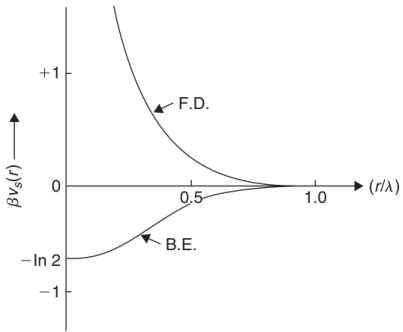
\includegraphics[width=0.36\textwidth]{images/chap5_m537b18d14f03bde19d574406a6848e1a.jpg}
\caption{一对遵循玻色-爱因斯坦统计或费米-狄拉克统计的粒子之间的统计势 \(v_{s}(r)\)。}
\label{fig:5_5.1}
\end{figure}

5.2. 证明：

\begin{equation}\tag{5.4.47}\label{eq:5.4.47}
\langle q | e ^{- \beta \hat { H} } | q ^{\prime} \rangle = \exp \left[ - \beta \hat { H } \left( - i \hbar \frac { \partial } { \partial q } , q \right) \right] \delta ( q - q ^{\prime} ) ,
\end{equation}

其中 \(\hat{H}(-i\hbar\,\partial/\partial q,q)\) 是系统在 \(q\) 表示下的哈密顿算符，该算符在形式上作用于狄拉克δ函数 \(\delta(q-q')\)。将δ函数展开为合适的形式，然后将这一结果应用于（i）自由粒子和（ii）线性谐振子。

推导出（i）自由粒子和（ii）线性谐振子在动量表示下的密度矩阵 \(\rho\)，并按照第 5.3 节的思路，研究其主要性质。

5.4. 以未对称化波函数（5.4.3）代替对称化波函数（5.5.7），研究自由粒子系统的密度矩阵及配分函数。表明，按照这一方法操作，既不会遇到吉布斯修正因子（1/N!），也不会出现粒子间的空间相关性。

5.5. 证明，在一阶近似下，由 \(N\) 个非相互作用、不可区分粒子组成的系统的配分函数可表示为：

\begin{equation}\tag{5.4.48}\label{eq:5.4.48}
Q _ { N } ( V , T ) = \frac { 1 } { N ! \lambda ^{3 N} } Z _ { N } ( V , T ) ,
\end{equation}

其中

\begin{equation}\tag{5.4.49}\label{eq:5.4.49}
Z _ { N } ( V , T ) = \int \exp \left\{ - \beta \sum _ { i < j } v _ { s } ( r _ { i j } ) \right\} d ^{3 N} r ,
\end{equation}

\(\nu_{s}(r)\) 为统计势（5.5.28）。进而计算该系统状态方程的一阶修正项。

5.6. 确定在标准状况下，氢、氦和氧的简并度判别式（\(n\lambda^{3}\)）的数值。估算这些量的相应温度范围，当其大小接近于 1 时，量子效应便开始变得显著。

5.7. 证明，一个由 \(N\) 个相互作用粒子组成的系统的量子力学配分函数，会趋近于经典形式。

\begin{equation}\tag{5.4.50}\label{eq:5.4.50}
Q _ { N } ( V , T ) = \frac { 1 } { N ! \, h ^{3 N} } \int e ^{- \beta E ( q , p )} d ^{3 N} q d ^{3 N} p
\end{equation}

随着平均热波长 \(\lambda\) 远远小于（i）粒子间平均距离 \((V/N)^{1/3}\)，以及（ii）粒子间势能的特征长度 \(r_0\) 时，系统的行为会趋于经典态。¹¹

5.8. 证明佩尔斯提出的以下定理。¹²

``若 \(\hat{H}\) 是给定物理系统的厄米哈密顿算符，而 \(\{\phi_{n}\}\) 是一组任意的正交波函数，且满足对称性要求以及边界条件\ldots\ldots{}''

问题的条件是，系统的配分函数满足以下不等式：

\begin{equation}\tag{5.4.51}\label{eq:5.4.51}
Q ( \beta ) \geq \sum _ { n } \exp \{ - \beta \langle \phi _ { n } | \hat { H } | \phi _ { n } \rangle \} ;
\end{equation}

当 \{\(\phi_{n}\)\} 构成哈密顿算符本身特征函数的完备正交集时，等号成立。

